\documentclass[12pt]{article}

\usepackage{geometry}

% Core packages
\usepackage{amsmath,amssymb}
\usepackage{tikz-cd}
\usepackage{multicol}
\usepackage{etoolbox}
\usepackage{fancyhdr}
\usepackage{setspace}
\usepackage{graphicx}
\usepackage{booktabs}
\usepackage[labelfont=bf]{caption}
\usepackage{amsmath}
\usepackage{optidef}

% biblio

% --- Bibliography Setup ---
\usepackage[
  backend=biber,
  style=authoryear,
  maxcitenames=2,
  dashed=false
]{biblatex}
\DeclareFieldFormat{titlecase}{#1}
\addbibresource{references.bib}
\pagestyle{fancy}
\graphicspath{{images/}}
\preto{\section}{\clearpage}
\setlength{\headheight}{15pt}
\renewcommand{\sectionmark}[1]{\markboth{#1}{}}

% Header styles
\fancyhf{}

% Header setup
\lhead{\nouppercase{\leftmark}}
\rhead{\thepage}

% Paragraphs
\setlength{\parindent}{0pt}
\setlength{\parskip}{1\baselineskip}

\title{Ports, Boats and Packages \\ \large A Two-Stage Optimisation of Urban Waterborne Logistics in Bergen}
\author{Olivier Deschênes}

\date{\today}

\begin{document}

\begin{titlepage}
  \centering
  \vspace*{\fill}

  {\textbf{\LARGE Ports, Boats and Packages}\par\vspace{-0.5\baselineskip}}
  {\large{\textit{A Two-Stage Optimisation of Urban Waterborne Logistics in Bergen}}\par}
  \vspace*{\fill}
  {\large{\textbf{Olivier Deschênes}}\par}
  \vspace*{\fill}
  {\bfseries
    {\large Jean-François Cordeau (HEC Montréal)\par\vspace{-0.5\baselineskip}}
    {\large Supervisors: Julio C. Góez (NHH)\par\vspace{-0.5\baselineskip}}
    {\large Stein W. Wallace (NHH)\par\vspace{-0.5\baselineskip}}
  }
  \vspace*{\fill}
  {\large MSc in Economics and Business Administration\par\vspace{-0.5\baselineskip}}
  {\large Energy, Natural Resources and the Environment\par}
  \vspace*{\fill}
  {\LARGE NORWEGIAN SCHOOL OF ECONOMICS\par}
  \vspace*{\fill}
  \vspace*{\fill}
  \begin{minipage}{1\textwidth}
    {\small This thesis was written as a part of the Master of Science in Economics and Business Administration at NHH. Please note that neither the institution nor the examiners are responsible -- through the approval of this thesis -- for the theories and methods used, or results and conclusions drawn in this work.\par}
  \end{minipage}
\end{titlepage}

\onehalfspacing

\section{Acknowledgements}

\section{Abstract}

\clearpage
\tableofcontents
\clearpage

\section{Test}

This is a test \parencite{smith2023}.
This is a test \parencite{smith2023, savelsbergh2016}.

Recent studies by \textcite{smith2023, savelsbergh2016} highlight the growing pressure of e-commerce on city infrastructure.

As demonstrated in Figure \ref{fig:demand_variance}, the maritime last-mile network experiences highly concentrated delivery volumes on certain days.

\begin{table}[htbp]
  \centering
  \caption{Daily parcel allocation and walking-time thresholds for candidate ports.}
  \label{tab:port_allocation_pro}

  \begin{tabular}{l c r}
    \toprule
    \textbf{Port Location} & \textbf{Walking Time (min)} & \textbf{Daily Parcels} \\
    \midrule
    Nordnes                & 5                           & 450                    \\
    Bryggen                & 8                           & 820                    \\
    Puddefjorden           & 12                          & 310                    \\
    \bottomrule
  \end{tabular}
\end{table}

this is a test for ref to As summarized in Table \ref{tab:port_allocation_pro}.

For a granular breakdown of the geographic coverage and spatial thresholds, see Appendix \ref{anx:bergen_map_annex}.

\begin{figure}[htbp]
  \centering
  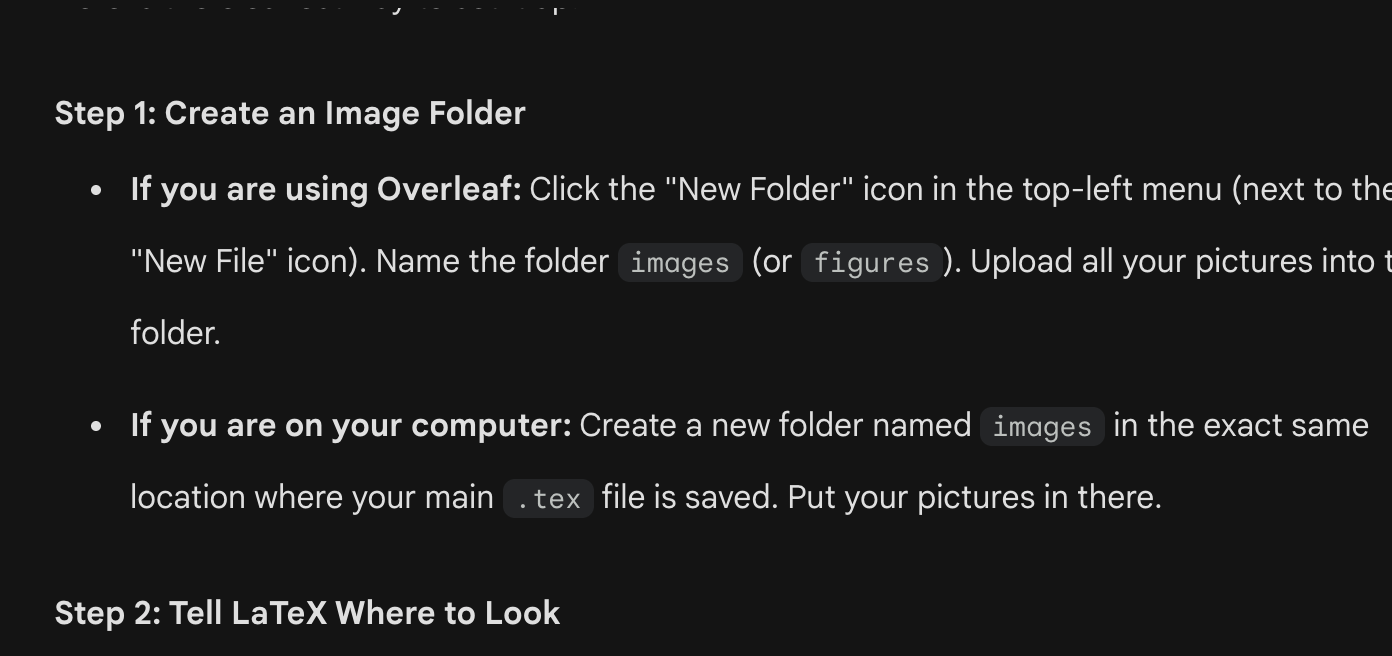
\includegraphics[width=0.8\textwidth]{image.png}
  \caption{Time-series visualization highlighting daily demand fluctuations across the network.}
  \label{fig:demand_variance}
\end{figure}

The total cost of the maritime last-mile network is calculated as follows:

\begin{equation}
  C_{total} = \sum_{i=1}^{n} (d_i \cdot w_i)
  \label{eq:total_cost}
\end{equation}

\begin{maxi!}
{x}{ \sum_{t=1}^{T} v_t x_t }{}{}
\addConstraint{d_t}{\le C_{max}, \quad \label{con:capacity}}{\text{(Daily Capacity Limit)}}
\end{maxi!}

As defined in \eqref{con:capacity}, the maritime network cannot exceed the daily threshold.

\begin{align}
  \sum_{j=1}^{n} x_{ij} & = 1 \label{eq:flow_out} \\
  \intertext{This ensures that every small port is visited exactly once per day. Furthermore, we must ensure flow conservation:}
  \sum_{i=1}^{n} x_{ij} & = 1 \label{eq:flow_in}
\end{align}

The objective function \eqref{eq:obj} minimizes the total routing costs across the network:
\begin{equation}
  \min Z = \sum_{i \in V} \sum_{j \in V} c_{ij} x_{ij} \label{eq:obj}
\end{equation}

Constraints \eqref{con:out} and \eqref{con:in} ensure that every small port is visited exactly once per day:
\begin{align}
  \sum_{j \in V} x_{ij} & = 1 &  & \forall i \in V \label{con:out} \\
  \sum_{i \in V} x_{ij} & = 1 &  & \forall j \in V \label{con:in}
\end{align}

Because daily deliveries to small ports exhibit highly volatile, spiky demand patterns, constraint \eqref{con:capacity_limit} enforces a strict upper bound on the daily vessel capacity $C_{max}$:
\begin{equation}
  d_t \le C_{max} \quad \forall t \in T \label{con:capacity_limit}
\end{equation}

\section{Introduction}
\subsection{Motivation}
dwadad
\subsection{Problem description}
\subsection{Research question}
\subsection{Thesis structure}

\section{Background}
\subsection{Urban Parcel Delivery and Last-Mile Logistics}
\subsection{Bergen as a Constrained Logistics Environment}
\subsection{Waterborne Transport as an Urban Freight Alternative}
\subsection{Facility Location and Accessibility}
\subsection{Vehicle Routing in Urban Freight Distribution}
\subsection{Demand Uncertainty and Scenario-Based Planning}
\subsection{Positioning of This Thesis}

\section{Data}
\subsection{Overview of Data Sources}
\subsection{PostNord Parcel Demand Data}
\subsection{Population and Household Data}
\subsection{OpenStreetMap Data}
\subsection{Candidate Port Locations}
\subsection{Distance and Travel Time Data}
\subsection{Demand Scenarios}
\subsection{Data Limitations}

\section{Methodology}
\subsection{Overall Methodological Framework}
\subsection{Port Location Model}
\subsubsection{Coverage Definition}
\subsubsection{Partial Set Covering Location Problem}
\subsubsection{Walking-Time Thresholds}
\subsection{Demand Allocation to Ports}
\subsubsection{Population-Based Allocation}
\subsubsection{Port-Level Parcel Demand}
\subsection{Boat Routing Model}
\clearpage
\subsubsection{Capacitated Vehicle Routing Problem}
\subsubsection{Split Delivery Vehicle Routing Problem}
\subsubsection{Capacity Constraints}
\subsubsection{Route Duration Constraints}
\subsubsection{Handling and Maneuvering Time}
\subsection{Scenario Design}
\subsubsection{Demand Scenarios}
\subsubsection{Boat Capacity Scenarios}
\subsubsection{Fleet Size Assumptions}

\section{Analysis}
\subsection{Port Location Results}
\subsection{Population Coverage Results}
\subsection{Port Demand Results}
\subsection{Boat Routing Results}
\subsection{Fleet Feasibility}
\subsection{Scenario Comparison}
\subsection{Sensitivity Analysis}

\section{Discussion}
\subsection{Interpretation of Results}
\subsection{Feasibility of Waterborne Parcel Delivery in Bergen}
\subsection{Operational Challenges}
\subsection{Demand and Capacity Limitations}
\subsection{Model Limitations}
\subsection{Practical Implications}
\subsection{Further Research}

\section{Conclusion}
\subsection{Summary of Findings}
\subsection{Answer to the Research Question}
\subsection{Final Remarks}

\clearpage
\printbibliography

\section{Appendix}
\appendix

\counterwithin{figure}{section}
\counterwithin{table}{section}

\subsection{Detailed Maps of Bergen Candidate Ports}
Here is the supplementary map showing the walking-time thresholds in greater detail.

\begin{figure}[h]
  \centering
  % Replace 'your_image.png' with your actual file name
  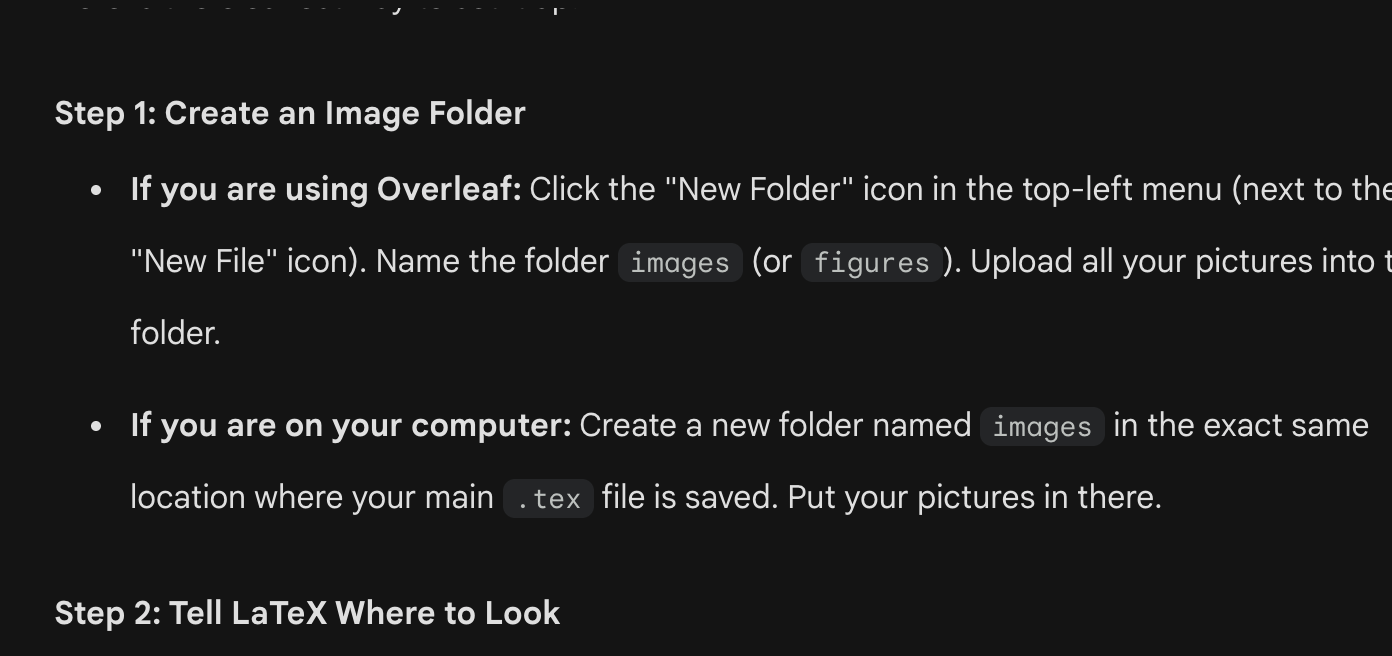
\includegraphics[width=0.8\textwidth]{image.png}
  \caption{Extended view of Bergen walking-time thresholds.}
  \label{anx:bergen_map_annex}
\end{figure}

\subsection{Extended PostNord Data Tables}

\end{document}

